%
%    Generated: VHDL to LaTeX
%    URL:       www.mamikon.net
%    Author:    Anna Bansaghi
%    Version:   1.0.5
%    Date:      12 March 2017
%
\documentclass[a4paper]{article}
\usepackage{tikz}
\usetikzlibrary{calc,arrows}
\makeatletter
\pgfdeclareshape{circuit}{
  \savedanchor\northeast{
    \pgfmathsetlength\pgf@x{\pgfshapeminwidth}
    \pgfmathsetlength\pgf@y{\pgfshapeminheight}
    \pgf@x=0.5\pgf@x
    \pgf@y=0.5\pgf@y}
  \savedanchor\southwest{
    \pgfmathsetlength\pgf@x{\pgfshapeminwidth}
    \pgfmathsetlength\pgf@y{\pgfshapeminheight}
    \pgf@x=-0.5\pgf@x
    \pgf@y=-2.65\pgf@y}
  \inheritanchorborder[from=rectangle]
  \anchor{center}{\pgfpointorigin}
  \anchor{north}{\northeast \pgf@x=0pt}
  \anchor{east}{\northeast \pgf@y=0pt}
  \anchor{south}{\southwest \pgf@x=0pt}
  \anchor{west}{\southwest \pgf@y=0pt}
  \anchor{north east}{\northeast}
  \anchor{north west}{\northeast \pgf@x=-\pgf@x}
  \anchor{south west}{\southwest}
  \anchor{south east}{\southwest \pgf@x=-\pgf@x}
  \anchor{text}{
    \pgfpointorigin
    \advance\pgf@x by -.5\wd\pgfnodeparttextbox
    \advance\pgf@y by -11.7375\ht\pgfnodeparttextbox
    \advance\pgf@y by +.5\dp\pgfnodeparttextbox}
\anchor{ina}{
  \pgf@process{\northeast}
  \pgf@x=-1\pgf@x
  \pgf@y=0.5\pgf@y}
\anchor{inb}{
  \pgf@process{\northeast}
  \pgf@x=-1\pgf@x
  \pgf@y=0.09999999999999998\pgf@y}
\anchor{inc}{
  \pgf@process{\northeast}
  \pgf@x=-1\pgf@x
  \pgf@y=-0.6000000000000001\pgf@y}
\anchor{ioa}{
  \pgf@process{\northeast}
  \pgf@y=0.5\pgf@y}
\anchor{ind}{
  \pgf@process{\northeast}
  \pgf@x=-1\pgf@x
  \pgf@y=-1.3\pgf@y}
\anchor{iob}{
  \pgf@process{\northeast}
  \pgf@y=-0.2\pgf@y}
\anchor{ine}{
  \pgf@process{\northeast}
  \pgf@x=-1\pgf@x
  \pgf@y=-2\pgf@y}
\anchor{inf}{
  \pgf@process{\northeast}
  \pgf@x=-1\pgf@x
  \pgf@y=-2.4\pgf@y}
\anchor{ing}{
  \pgf@process{\northeast}
  \pgf@x=-1\pgf@x
  \pgf@y=-2.8\pgf@y}
\anchor{inh}{
  \pgf@process{\northeast}
  \pgf@x=-1\pgf@x
  \pgf@y=-3.2\pgf@y}
\anchor{ini}{
  \pgf@process{\northeast}
  \pgf@x=-1\pgf@x
  \pgf@y=-3.6\pgf@y}
\anchor{inj}{
  \pgf@process{\northeast}
  \pgf@x=-1\pgf@x
  \pgf@y=-4\pgf@y}
\anchor{outa}{
  \pgf@process{\northeast}
  \pgf@y=-0.9000000000000001\pgf@y}
\anchor{ioc}{
  \pgf@process{\northeast}
  \pgf@y=-1.3\pgf@y}
\anchor{ink}{
  \pgf@process{\northeast}
  \pgf@x=-1\pgf@x
  \pgf@y=-4.699999999999999\pgf@y}
\anchor{inl}{
  \pgf@process{\northeast}
  \pgf@x=-1\pgf@x
  \pgf@y=-5.1\pgf@y}
\backgroundpath{
  \pgfpathrectanglecorners{\southwest}{\northeast}
  \begingroup
    \tikzset{labels}
    \tikz@textfont
  \endgroup}}
\tikzset{add font/.code={\expandafter\def\expandafter\tikz@textfont\expandafter{\tikz@textfont#1}}}
\tikzset{labels/.style={font=\sffamily\scriptsize}}
\tikzset{every circuit node/.style={draw,minimum width=5cm,minimum height=2.5cm,very thick,inner sep=1mm,outer sep=0pt,cap=round,add font=\sffamily\bfseries}}
\makeatother
\begin{document}
\begin{figure}[htb]
\centering
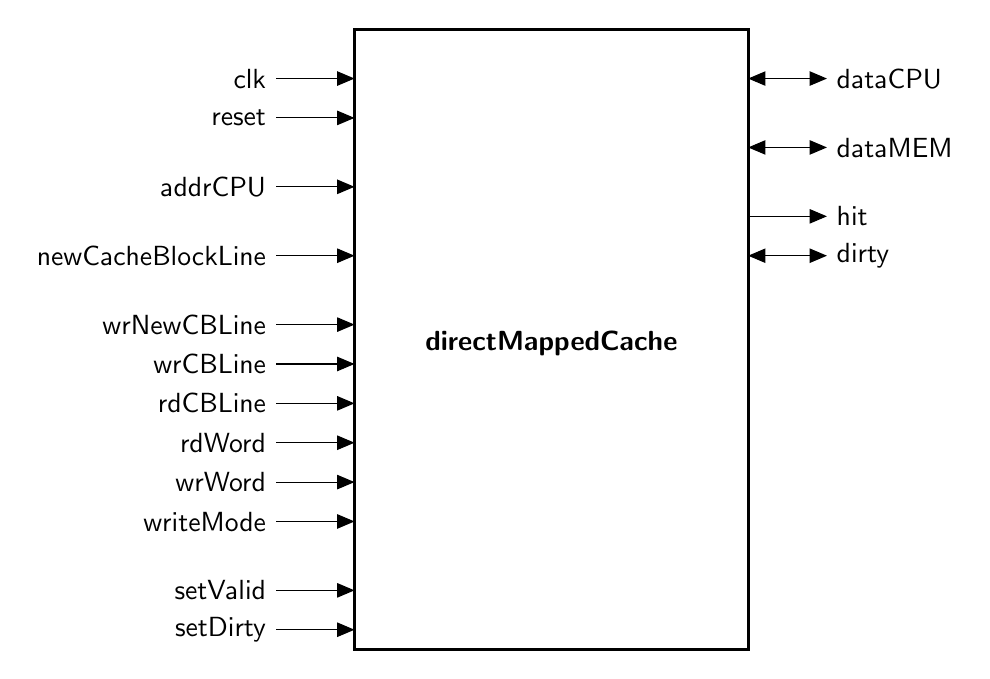
\begin{tikzpicture}[font=\sffamily,>=triangle 45]
  \node [shape=circuit] (item) at (0,0) {directMappedCache};
  \draw [<-] (item.ina) node [anchor=west,labels] {} -- +(-1,0) node [anchor=east] {clk};
  \draw [<-] (item.inb) node [anchor=west,labels] {} -- +(-1,0) node [anchor=east] {reset};
  \draw [<-] (item.inc) node [anchor=west,labels] {} -- +(-1,0) node [anchor=east] {addrCPU};
  \draw [<->] (item.ioa) node [anchor=east,labels] {} -- +(1,0) node [anchor=west] {dataCPU};
  \draw [<-] (item.ind) node [anchor=west,labels] {} -- +(-1,0) node [anchor=east] {newCacheBlockLine};
  \draw [<->] (item.iob) node [anchor=east,labels] {} -- +(1,0) node [anchor=west] {dataMEM};
  \draw [<-] (item.ine) node [anchor=west,labels] {} -- +(-1,0) node [anchor=east] {wrNewCBLine};
  \draw [<-] (item.inf) node [anchor=west,labels] {} -- +(-1,0) node [anchor=east] {wrCBLine};
  \draw [<-] (item.ing) node [anchor=west,labels] {} -- +(-1,0) node [anchor=east] {rdCBLine};
  \draw [<-] (item.inh) node [anchor=west,labels] {} -- +(-1,0) node [anchor=east] {rdWord};
  \draw [<-] (item.ini) node [anchor=west,labels] {} -- +(-1,0) node [anchor=east] {wrWord};
  \draw [<-] (item.inj) node [anchor=west,labels] {} -- +(-1,0) node [anchor=east] {writeMode};
  \draw [->] (item.outa) node [anchor=east,labels] {} -- +(1,0) node [anchor=west] {hit};
  \draw [<->] (item.ioc) node [anchor=east,labels] {} -- +(1,0) node [anchor=west] {dirty};
  \draw [<-] (item.ink) node [anchor=west,labels] {} -- +(-1,0) node [anchor=east] {setValid};
  \draw [<-] (item.inl) node [anchor=west,labels] {} -- +(-1,0) node [anchor=east] {setDirty};
\end{tikzpicture}
\caption{Entity of directMappedCache}
\end{figure}
\end{document}
